\documentclass[a4papper]{article}
\title{}
\usepackage{color}
\usepackage{ctex}
\usepackage{amssymb}
\usepackage{amsmath}
\usepackage{upgreek}
\usepackage{mathtools}
\usepackage{subfigure}
\usepackage{float}
\usepackage{indentfirst} %段落自动缩进
\usepackage{geometry}  %页边距
\usepackage{subfigure}
\usepackage{booktabs}
\usepackage{txfonts}
\usepackage{setspace}
\usepackage{CJK,CJKnumb}
\usepackage[colorlinks, citecolor=black, pagebackref,linkcolor=black]{hyperref}%backref表示反向引用,点击文献名称可以返回引用页
\usepackage{fancyhdr} % 添加页眉页脚
\pagestyle{fancy}%设置页眉和页脚
\lhead{}
\chead{}
\lfoot{}
\cfoot{}
\rfoot{\thepage}
%\renewcommand{\headrulewidth}{0pt} %改为0pt即可去掉页眉下面的横线
%\renewcommand{\footrulewidth}{0pt} %改为0pt即可去掉页脚上面的横线 0.4pt
\usepackage[raggedleft]{titlesec} %设置标题
\usepackage{textcomp}

\newcommand{\kai}{\CJKfamily{kai}} 
\newcommand{\upcite}[1]{\textsuperscript{\textsuperscript{\cite{#1}}}}%文献上标

\renewcommand{\figurename}{Fig.}
\renewcommand{\contentsname}{目录}
\renewcommand{\thefigure}{\arabic{figure}}
\renewcommand{\tablename}{Table 1.}
\renewcommand{\thesubfigure}{(\alph{subfigure}}


\titleformat{\section}{\center\Huge\bfseries}{\thesection .}{.5em}{}%定义section样式
\titleformat{\subsection}{\raggedright\Large\bfseries}{\thesubsection .}{.5em}{}
\titleformat{\subsubsection}{\raggedright\large\bfseries}{\thesubsubsection .}{.5em}{}

\bibliographystyle{plain}

\geometry{left=3cm,top=3cm,bottom=4cm,right=3cm}
\title{第四周}

\author{网络流量分类和特征提取研究内容小结\\\\
Wu You\\ 
}
\begin{document}
\maketitle
\tableofcontents
\thispagestyle{empty}%取消此页页眉和页脚
\newpage
\setcounter{page}{1}%将此页页码计数设置为1
\setcounter{section}{0}%在此处将section计数设置为0,下个section将为1号
\section{课题背景介绍}
\subsection{当前网络环境分析}
\par\setlength{\parindent}{2em} %设置段落缩进
由于互联网技术发展迅速,同时也为国家发展带来了巨大的经济效益,我国的互联网规模在一段时期内还将不断扩大。而随着互联网的不断普及,用户人数不断增加,同时产生了多种类的新型网络应用,网络已经覆盖了生产生活的各个方面,社会发展对网络的依赖性也逐渐增强。而网络规模的告诉发展也带来一定问题,首先一些使用新型的网络应用如基于P2P或VoIP的软件对于网络的占用率较高,影响其他网络应用的运行;其次随着电子商务的兴起,网络中信息价值不断提高,导致网络安全问题日益突出;最后,互联网信息扩散十分迅速,为不良信息的传播提供了条件。\cite{林冠洲2011网络流量识别关键技术研究}可以看出,加强对网络流量的监督和管理是十分重要的。
\par\setlength{\parindent}{2em} %设置段落缩进
当前网络环境有流量大、种类多、发展快的特点,无论是网络的监督管理,还是安全防护,在全流量的基础上进行无疑是事倍功半,迫切需要对流量进行分类以进行有针对性的工作,因此网络流量的分类技术需要不断升级以应对日益复杂的网络环境。流量分类识别是进行各项网络分析工作的第一步,同时,在该方向上的研究成果也可以部分迁移至后续的分析步骤中,故流量分类技术的研究对于当前社会具有重大意义。
\subsection{流量分类的主要工作内容}
\par\setlength{\parindent}{2em} %设置段落缩进
有关网络流量分类的研究可以分为流量数据采集和预处理、特征的提取、算法的选择与改进以及分类系统的部署等问题。其中,行业内进行数据采集的方法已经较为完善,并且有多种数据集可用于研究,但对于其后的特征提取问题,目前还不存在十分完美的解决方案。作为流量分析的重要环节,流量特征选取对于分类性能有着决定性的作用,其中不仅需要考虑耗时、准确率等问题,特征选取策略的及时更新也十分重要,因此需要研究流量特征的自动提取方法。图1中给出了流量分类的主要工作过程,并分析了特征提取技术的研究内容,理想的分类系统可以在较少的人工指导下运行,并保持良好的分类性能。
\[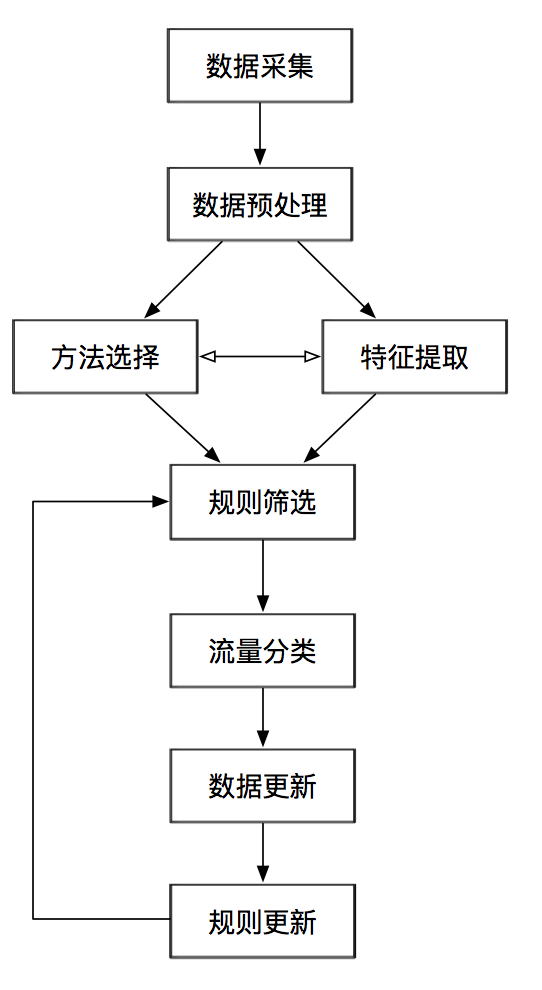
\includegraphics[width=4cm,height=8cm]{../../Figures/Procedure_of_Flow_Classification.png}\]%插入图片
\begin{center}
图1 流量分类工作流程 %图片标注(需解决自动序号问题)
\end{center}

\section{网络流量分析技术}
\par\setlength{\parindent}{2em} %设置段落缩进
网络流量分类是根据不同网络应用流量的特点,实现网络流量的对比、分类,在网络流量管理、信息监测或者网络安全防护工作上,流量分类都是一项重要技术手段。流量特征的提取,需要依据算法的选择,而算法的选择,取决于流量分析的具体方式,三者相互制约。根据分析层面可以将流量分析技术分为三类,即基于端口的分析、深度包检测(Deep Packet Inspection, DPI)以及深度流检测(Deep Flow Inspection, DFI)。
\subsection{基于端口的流量识别}
\par\setlength{\parindent}{2em} %设置段落缩进
早期互联网应用种类较少,不同协议的应用只需根据标准端口号即可进行区分,但互联网环境日渐复杂,出现了多种端口伪装技术,同时新兴的互联网协议,如P2P协议使用了动态端口技术导致该方法的准确率大大降低,目前只能作为辅助分析手段。\cite{柏骏2013实时网络流量分类研究综述}
\subsection{基于深度包检测的流量识别}
\par\setlength{\parindent}{2em} %设置段落缩进
深度包检测技术是一种基于数据包载荷的流量分析技术。由于相同应用的数据包内容有一定的相似性,可以从数据包的内容中提取一定的特征作为规则,并建立规则库,通过内容匹配来进行流量分类。这种方法的优点是识别精度较高,但是由于需要获取数据包内容,涉及了用户隐私问题,同时在高速网络中,分析的实时性无法得到保证。现今网络环境迅速变化,依赖人工建立规则库的开销巨大,且无法对规则库进行及时的更新,而大量的规则也会引起分析速度下降等问题,因此现在DPI的研究方向除了算法识别精度的提升外,还包括算法运行速度的提升以及规则的筛选问题。
\subsection{基于深度流检测的流量识别}
\par\setlength{\parindent}{2em} %设置段落缩进
深度流检测技术是一种基于网络流量整体统计特征的分析技术。该技术主要依赖机器学习算法,可以实现流量的自动、准确分类。但是由于需要提取网络流的整体特征,很难做到流量的实时分析,且训练得到的模型在处理未知类型流量时无法拥有良好的健壮性。目前针对该技术的研究主要方向有算法的选择、对比和优化,特征的有效选取以及未知流量的识别等。
\par\setlength{\parindent}{2em} %设置段落缩进
当前的机器学习算法按照样本数据的形式,可分为无监督学习、有监督学习以及半监督学习。无监督学习算法的主要作用是对数据进行聚类,这类算法不需要初始数据的分类标签,可以自动将数据进行划分,但无法得到数据的类别,常见的无监督学习算法有K均值、DBSCAN、谱聚类等。有监督学习算法要求样本数据带有标签,这类算法性成一种从数据属性到数据类别的映射模型,并利用该模型对未来数据进行分类,常见的有监督学习算法有决策树、支持向量机(Support Vector Machine)、贝叶斯方法以及神经网络等。虽然有监督学习算法可以实现数据的有效分类,但对初始数据的标定工作难度较大,半监督学习则可以有效解决这一问题。半监督学习算法首先对数据进行初始聚类,之后再使用少量已标定数据确定类别信息。
\par\setlength{\parindent}{2em} %设置段落缩进
目前基于机器学习的流量分类,已成为国内外研究的研究重点。文献\cite{Moore:2005:ITC:1071690.1064220}中采用了改机的朴素贝叶斯算法进行流量分类,通过在概率公式中引入改进的核函数,结合一定的特征选择策略,使算法准确率达到了95\%以上,作者在另一篇文章\cite{moore2013discriminators}中介绍了所使用的249种流量特征,并公开了其所使用的数据集。文献\cite{林冠洲2011网络流量识别关键技术研究}中使用了一种基于K均值改进的半监督学习算法,作者改进了K均值算法的初始中心选择策略,与传统K均值算法和KKZ算法相比,性能有所提高,但仍不能保证其实时性,并且在算法性能的对比环节缺少与有监督学习算法的对照,无法体现文中算法的优势。同时,作者也没有解决参数选取、特征选取等问题。文献\cite{牟澄2014互联网流量特征智能提取关键技术研究}中,使用了传统反向传播(Back Propagation,BP)神经网络对数据进行分类,但相对网络结构较为简单,并且未对网络结构做出解释。文献\cite{彭立志2015基于机器学习的流量识别关键技术研究}中使用了基于柔性神经树(Flexible Neuron Tree)的算法,并使用PIPE算法优化FNT的树结构,同时使用粒子算法(PSO)来进行FNT的参数优化。
\par\setlength{\parindent}{2em} %设置段落缩进
无论DPI技术还是DFI技术,都存在一些共同的问题值得研究。例如数据方面可能会存在样本不均文献\cite{彭立志2015基于机器学习的流量识别关键技术研究}中提出了样本数据不均衡的问题,并提出了一种模型来改善此问题。为了保证分类系统实时性和健壮性,算法的运行效率以及自我更新能力也需要深入研究。还有一些算法本身带有参数,使用这类算法时还需考虑参数选择对分类效果的影响。由于两种技术各有其弊端,也有人提出使用混合的流量识别方法,从而更好地贴合应用场景,这也是目前流量分类研究的发展趋势。
\section{网络流量特征提取}
\par\setlength{\parindent}{2em} %设置段落缩进
特征的提取对于流量识别的速度、精度等有直接影响,人工特征提取的方式开支较大,且有效性和时效性无法得到保证,故自动特征提取成为现在研究的重点。基于DPI和DFI的流量分析所使用的特征有很大区别,因此相应的特征提取技术也有所不同。
\subsection{DPI分析特征提取}
\par\setlength{\parindent}{2em} %设置段落缩进
基于DPI的流量分析主要使用了流量内容的模式特征,除字符串以外,还可以包括比特串、正则表达式以及序列模式等,这类特征的提取方法是利用数据挖掘算法分析数据包的内容字段与其流量类别之间的关联度,并提取出关联度较高的部分。下面将介绍几种用于模式特征提取的方法。
\par\setlength{\parindent}{2em} %设置段落缩进
文献\cite{林冠洲2011网络流量识别关键技术研究}中使用了一种基于序列模式挖掘的特征提取方法,该算法是经典PrefixSpan算法的改进,直接在数据包的十六进制数序列中进行挖掘,通过模式增长的方式来生成连续序列模式。其中还使用了偏移属性约束,在一定程度上减少了算法的计算量。但该算法没有考虑规则库的筛选和更新问题,文中提出可使用\emph{增量序列模式挖掘}的方法来实现规则库的更新。文献\cite{马婧2012网络流量特征提取与流量识别研究}中在AutoSig算法的基础上进行了一定修改,提出了一种自动协议指纹挖掘算法以用于P2P流量的特征提取。实验结果表明该算法可以挖掘出人工未能总结出的协议指纹。文献\cite{牟澄2014互联网流量特征智能提取关键技术研究}中使用了固定比特流算法进行流量特征提取,并进行了规则集的筛选工作,结果表明该算法运行时间相对于类Apriori算法和类SPADE算法有明显缩短。文中还详细介绍了数据的预处理和规则的后处理策略,有一定参考价值。最后,作者还提出可以使用PCA的方法来缩短特征提取时间,并精简规则库。
\subsection{DFI分析特征提取}
\par\setlength{\parindent}{2em} %设置段落缩进
基于DFI的流量分析主要使用了流量整体的统计特征,在特征的选取方面,Moore提出了针对TCP网络流量的249种统计特征,利用这些特征,只需了解TCP数据包的头部信息即可进行分类\cite{moore2013discriminators},这对于算法的实时性有重大意义。可以看出DFI技术所面对的主要是特征的选择,而不是提取问题,合理的特征选择可以提高算法的精度、速度,从而实现流量的实时检测。下面将介绍几种统计特征选取的方法。
\par\setlength{\parindent}{2em} %设置段落缩进
文献\cite{武建华2009基于关联规则的特征选择算法}介绍了一种基于关联规则的特征选择算法,该算法基于Apriori算法原理,首先寻找各个特征取值与类别之间的关联规则,并按照长度最短、置信度最大、支持度最大的顺序进行规则挑选,从而提取出可以对数据进行有效分类的属性,作为分类算法的特征。该算法在样本量较大时运行速度较慢。文献\cite{牟澄2014互联网流量特征智能提取关键技术研究}中,首先确定了37个特征,将训练模型所使用的特征数限定为3个,并利用神经网络算法对所有组合的分类效果进行比对,找到了其中最有效的10个特征组合和10个无效特征组合。结果表明,有效组合与无效组合所包含特征的重合率很低,说明了\emph{单个特征的有效性不会因为组合的变化而有太大波动}。但文中并未阐述\emph{为何将特征数限定为3个,也没有提出一种有效的特征选择策略},仅仅遍历的所有可能的组合得出结果,与实际应用仍有较大差距;同时,作者只利用了BP神经网络进行测试,结果可能存在偏差。文献\cite{彭立志2015基于机器学习的流量识别关键技术研究}中基于柔性神经树(Flexible Neuron Tree,FNT)进行了流量的特征选择与识别。
\section{总结}
\par\setlength{\parindent}{2em} %设置段落缩进
随着互联网规模的迅速扩大,出现了许多新型网络应用,网络安全问题也日益突出,这给网络的管理工作带来了挑战,对网络流量进行有效分类可以帮助有针对性地进行各类管理工作。流量特征的提取方法直接决定了分类的精度和效率,而由于当前网络的多边性,基于人工进行特征提取的方法已经无法满足工作需求,因此需要研究特征的自动提取技术,最终目标是实现流量的自动、准确分类,并确保分类系统的实时更新以保持其健壮性。本周总结了网络流量分类的组成内容,并总结了部分相关研究工作的亮点与不足。接下来计划首先从DPI方法入手,通过序列模式挖掘算法实现数据分类,深入理解算法,并继续阅读文献,寻找研究方向。

%\[\includegraphics[width=10cm]{../../Desktop/sb/1}\] 图片
\bibliography{../../Reference/reference_flow_analysis.bib}
\end{document}